\chapter{非线性最小二乘法}

\section{非线性最小二乘法的定义}

\begin{problem}
    $ f_{1}(x), \ldots, f_{m}(x) $ 是可微函数;

    优化目标: $$ \min _{x} \sum_{i=1}^{m}\left(f_{i}(x)\right)^{2} $$

\end{problem}

\begin{problem}
    \label{pbl:non-linear-least-squares}
    设函数 $ f(x): \mathbb{R}^{n} \rightarrow \mathbb{R}^{m} $ ,其第 $ i $ 个分量为函数 $ f_{i}(x)$

    则有
    $$
    f(x)=\left[\begin{array}{c}
    f_{1}(x) \\
    f_{2}(x) \\
    \vdots \\
    f_{m}(x)
    \end{array}\right]
    $$

    优化目标
    $$ \min _{x} \sum_{i=1}^{m}\left(f_{i}(x)\right)^{2}=\|f(x)\|_{2}^{2} $$
\end{problem}


如果 $ f(x)=A x-b $ ,问题简化为(线性)最小二乘问题。

\subsection{例子:距离测量定位}

\begin{problem}
    向量 $ x_{e x} $ 表示二维或三维中的未知位置,通过测量到的已知点 $ a_{1}, \cdots, a_{m} $ 的距离来估计 $ x_{e x} $ 

    $$
    \rho_{i}=\left\|x_{e x}-a_{i}\right\|_{2}+v_{i}, \quad i=1, \cdots, m
    $$

    其中 $ v_{i} $ 是测量误差。
\end{problem}

非线性最小二乘法估计:通过最小化估计 $ \hat{x} $的位置

$$
\min _{x} \sum_{i=1}^{m}\left(\left\|x-a_{i}\right\|_{2}-\rho_{i}\right)^{2}=\|f(x)\|_{2}^{2}
$$

函数$ f_{i}(x)=\left\|x-a_{i}\right\|_{2}-\rho_{i} $ 是 $ f(x) $ 的 $ i $ 个分量。

% todo (2021-12-09 17:19): figure

\subsection{例子:多个相机视图定位}

\begin{remark}
    这个例子与遥感卫星成像等有关。
\end{remark}

建立一个理想的相机模型,由参数 $ A \in \mathbb{R}^{2 \times 3}, b \in \mathbb{R}^{2}, c \in \mathbb{R}^{3}, d \in \mathbb{R} $ 来描述。相机及其位置和方向用 $ A , b , c , d $ 来刻画。

目标位置 $ x \in \mathbb{R}^{3} $ 在二维平面图像投影位置 $ x^{\prime} \in \mathbb{R}^{2} $ 。

$$
x^{\prime}=\frac{1}{c^{T} x+d}(A x+b)
$$

如果物体在摄像机前面,则 $ c^{T} x+d>0 $ 。

\begin{problem}
    位于 $ x_{e x} $ 位置的物体由 $ l $ 个相机观察(由 $ A_{i}, b_{i}, c_{i}, d_{i} $ 描述),目标在相机图像平面上位置 $ y_{i} \in \mathbb{R}^{2} $

    $$
    y_{i}=\frac{1}{c_{i}^{T} x_{e x}+d_{i}}\left(A_{i} x_{\alpha x}+b_{i}\right)+v_{i}
    $$

    $ v_{i} $ 为测量误差或量化误差。目的是从 $ l $ 个观测点 $ y_{1}, \ldots, y_{l} $ 来估计三维位置 $ x_{e x} $ 。
\end{problem}


使用非线性最小二乘法估计
$$
\min _{x} \sum_{i=1}^{l}\left\|\frac{1}{c_{i}^{T} x+d_{i}}\left(A_{i} x+b_{i}\right)-y_{i}\right\|_{2}^{2}
$$

这是关于 $ m=2 l $ 的非线性最小二乘法问题, $ \left(y_{i}\right)_{j} $ 是 $ y_{i} $ 的第 $ j $ 个 分量:
$$
f_{i}(x)=\frac{\left(A_{i} x+b_{i}\right)_{1}}{c_{i}^{T} x+d_{i}}-\left(y_{i}\right)_{1}, \quad f_{l+i}(x)=\frac{\left(A_{i} x+b_{i}\right)_{2}}{c_{i}^{T} x+d_{i}}-\left(y_{i}\right)_{2}
$$

\subsection{例子:模型拟合}

\begin{problem}
$$
\min _{\theta} \sum_{i=1}^{N}\left(\hat{f}\left(x^{(i)}, \theta\right)-y^{(i)}\right)^{2}
$$

$ \left(x^{(i)}, y^{(i)}\right), i=1, \cdots, N $ 表示样本。设函数 $ \hat{f}(x, \theta) $ 的参数 $ \theta = \left(\theta_{1}, \ldots, \theta_{p}\right) $。最小化的目标是估计函数参数 $ \theta $。
\end{problem}

假设函数 $ \hat{f}(x, \theta) $ 关于 $ \theta $ 的线性函数
$$
\hat{f}(x, \theta)=\theta_{1} f_{1}(x)+\cdots+\theta_{p} f_{p}(x)
$$

当然 $ \hat{f}(x, \theta) $ 也可以是关于 $ \theta $ 的非线性函数。

\begin{example}
    有四个变量 $ \theta_{1}, \theta_{2}, \theta_{3}, \theta_{4} $ 的非线性最小二乘问题:
$$
\min _{\theta} \sum_{i=1}^{N}\left(\theta_{1} e^{\theta_{2} x(i)} \cos \left(\theta_{3} x^{(i)}+\theta_{4}\right)-y^{(i)}\right)^{2}
$$

% todo (2021-12-09 19:15): figure
\end{example}

\subsection{例子:正交距离回归}

正交距离回归目标: 最小化 $ \hat{f}(x, \theta) $ 图中数据点到曲线的均方距离。 

例子: 三次多项式的正交距离回归:
$$
\hat{f}(x, \theta)=\theta_{1}+\theta_{2} x+\theta_{3} x^{2}+\theta_{4} x^{3}
$$

% todo (2021-12-09 19:16): figure

\subsection{非线性最小二乘法}

\begin{problem}
    $$
\min _{\theta, u^{(i)}} \sum_{i=1}^{N}\left(\left(\hat{f}\left(u^{(i)}, \theta\right)-y^{(i)}\right)^{2}+\left\|u^{(i)}-x^{(i)}\right\|_{2}^{2}\right)
$$

这个模型需要优化参数 $ \theta $ 和 $ {N} $ 个点 $ u^{(i)} $。
\end{problem}

第 $ i $ 项为数据点 $ \left(x^{(i)}, y^{(i)}\right) $ 到点 $ \left(u^{(i)}, \hat{f}\left(u^{(i)}, \theta\right)\right) $ 距离的平方。

\begin{FigureCenter}{优化模型的几何意义}
    

\tikzset{every picture/.style={line width=0.75pt}} %set default line width to 0.75pt        

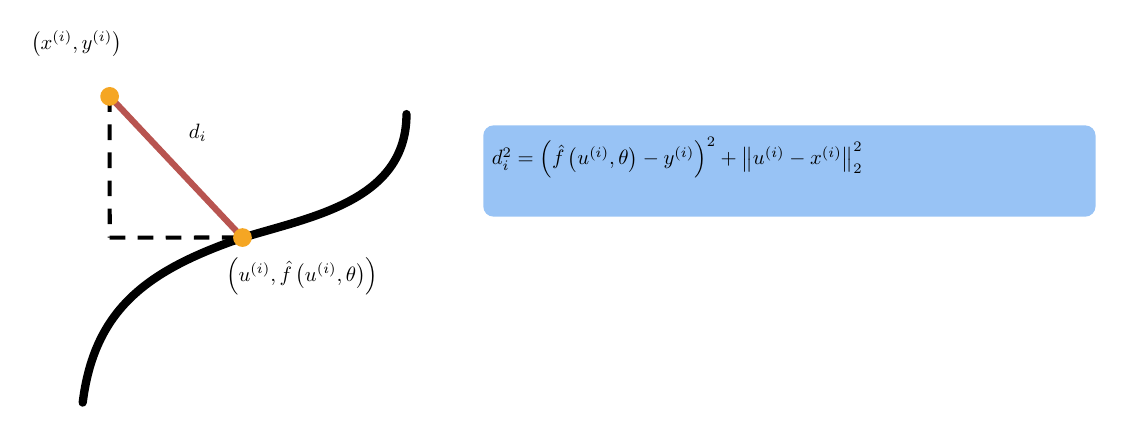
\begin{tikzpicture}[x=0.75pt,y=0.75pt,yscale=-1,xscale=1]
%uncomment if require: \path (0,300); %set diagram left start at 0, and has height of 300

%Shape: Free Drawing [id:dp5002881259079404] 
\draw  [color={rgb, 255:red, 0; green, 0; blue, 0 }  ][line width=3] [line join = round][line cap = round] (63.01,245.57) .. controls (68.41,202.42) and (91.96,183.67) .. (133.01,168.57) .. controls (164.12,157.14) and (219.01,152.23) .. (219.01,106.57) ;
%Straight Lines [id:da19530315633268636] 
\draw [color={rgb, 255:red, 184; green, 84; blue, 80 }  ,draw opacity=1 ][line width=2.25]    (75.99,98.05) -- (139.99,166.05) ;
%Straight Lines [id:da6781226747978477] 
\draw [line width=1.5]  [dash pattern={on 5.63pt off 4.5pt}]  (75.99,98.05) -- (76.01,166.1) ;
%Straight Lines [id:da3955370838358767] 
\draw [line width=1.5]  [dash pattern={on 5.63pt off 4.5pt}]  (76.01,166.1) -- (139.99,166.05) ;
%Shape: Circle [id:dp03457846112388152] 
\draw  [color={rgb, 255:red, 245; green, 166; blue, 35 }  ,draw opacity=1 ][fill={rgb, 255:red, 245; green, 166; blue, 35 }  ,fill opacity=1 ] (135.98,166.05) .. controls (135.98,163.84) and (137.77,162.04) .. (139.99,162.04) .. controls (142.2,162.04) and (144,163.84) .. (144,166.05) .. controls (144,168.27) and (142.2,170.06) .. (139.99,170.06) .. controls (137.77,170.06) and (135.98,168.27) .. (135.98,166.05) -- cycle ;
%Shape: Circle [id:dp15280043442217006] 
\draw  [color={rgb, 255:red, 245; green, 166; blue, 35 }  ,draw opacity=1 ][fill={rgb, 255:red, 245; green, 166; blue, 35 }  ,fill opacity=1 ] (71.98,98.05) .. controls (71.98,95.84) and (73.77,94.04) .. (75.99,94.04) .. controls (78.2,94.04) and (80,95.84) .. (80,98.05) .. controls (80,100.27) and (78.2,102.06) .. (75.99,102.06) .. controls (73.77,102.06) and (71.98,100.27) .. (71.98,98.05) -- cycle ;

% Text Node
\draw (37,65.44) node [anchor=north west][inner sep=0.75pt]  [xscale=0.75,yscale=0.75]  {$\left( x^{( i)} ,y^{( i)}\right)$};
% Text Node
\draw (113,110.4) node [anchor=north west][inner sep=0.75pt]  [xscale=0.75,yscale=0.75]  {$d_{i}$};
% Text Node
\draw  [color={rgb, 255:red, 0; green, 0; blue, 0 }  ,draw opacity=0 ][fill={rgb, 255:red, 152; green, 195; blue, 245 }  ,fill opacity=1 ]  (256,117) .. controls (256,114.24) and (258.24,112) .. (261,112) -- (546,112) .. controls (548.76,112) and (551,114.24) .. (551,117) -- (551,151) .. controls (551,153.76) and (548.76,156) .. (546,156) -- (261,156) .. controls (258.24,156) and (256,153.76) .. (256,151) -- cycle  ;
\draw (259,116.4) node [anchor=north west][inner sep=0.75pt]  [xscale=0.75,yscale=0.75]  {$d_{i}^{2} =\left(\hat{f}\left( u^{(i)} ,\theta \right) -y^{(i)}\right)^{2} +\left\Vert u^{(i)} -x^{(i)}\right\Vert _{2}^{2}$};
% Text Node
\draw (131,174.4) node [anchor=north west][inner sep=0.75pt]  [xscale=0.75,yscale=0.75]  {$\left( u^{(i)} ,\hat{f}\left( u^{(i)} ,\theta \right)\right)$};


\end{tikzpicture}
\end{FigureCenter}

通过 $ u^{(i)} $ 与图中点 $ \left(x^{(i)}, y^{(i)}\right) $ 的平方距离来最小化 $ d_{i}^{2} $。最小化 $ \sum_{i} d_{i}^{2} $ ,即通过 $ u^{(1)}, \ldots, u^{(N)} $ 和 $ \theta $ 来最小化均方距离。

\subsection{二分类}

二分类的目标函数为 $ \hat{f}(x, \theta)=\operatorname{sign}\left(\theta_{1} f_{1}(x)+\theta_{2} f_{2}(x)+\cdots+\theta_{p} f_{p}(x)\right) $ 


\begin{problem}[二分类问题]
    $$
\min _{\theta} \sum_{i=1}^{N}\left(\phi\left(\theta_{1} f_{1}\left(x^{(i)}\right)+\cdots+\theta_{p} f_{p}\left(x^{(i)}\right)\right)-y^{(i)}\right)^{2}
$$

$ \left(x^{(i)}, y^{(i)}\right) $ 是数据点, $ y^{(i)} \in\{-1,1\} $ 。 $ \phi(u) $ 是sigmoid函数,它是 $\operatorname{sign} (u) $ 函数的一个可微的近似函数。
$$
\phi(u)=\frac{e^{u}-e^{-u}}{e^{u}+e^{-u}}
$$
\end{problem}


通过计算 $ \theta $ 来求解非线性最小二乘问题,\textbf{大概率}能得到良好的结果。



\section{梯度}

\subsection{Gradient and Directional Derivative}

\begin{definition}[$\mathbb{R}^{n} \rightarrow \mathbb{R}$函数$g$的梯度]
    可微函数 $ g: \mathbb{R}^{n} \rightarrow \mathbb{R} $ 在 $ z \in \mathbb{R}^{n} $ 的梯度(gradient)为

$$
\nabla g(z)=\left[\begin{array}{c}
\frac{\partial g}{\partial x_{1}}(z) \\
\frac{\partial g}{\partial x_{2}}(z) \\
\cdots \\
\frac{\partial g}{\partial x_{n}}(z)
\end{array}\right]
$$
\end{definition}

\begin{definition}[$g$在$z$附近的仿射近似(一阶泰勒公式,线性化)]
    $$ \begin{aligned} \hat{g}(x) &=g(z)+\frac{\partial g}{\partial x_{1}}(z)\left(x_{1}-z_{1}\right)+\cdots+\frac{\partial g}{\partial x_{n}}(z)\left(x_{n}-z_{n}\right) \\ &=g(z)+\nabla g(z)^{T}(x-z) \end{aligned} $$
\end{definition}

\begin{definition}[Directional Derivative]
    For given $ z $ and nonzero $ v $, define $ h(t)=g(z+t v) $

   The derivative of $ h $ at $ t=0 $
$$
\begin{aligned}
h^{\prime}(0) &=\frac{\partial g}{\partial x_{1}}(z) v_{1}+\frac{\partial g}{\partial x_{2}}(z) v_{2}+\cdots+\frac{\partial g}{\partial x_{n}}(z) v_{n} \\
&=\nabla g(z)^{T} v
\end{aligned}
$$

This is called the \term{directional derivative} of $ g $ (at $ z $, in the direction $ v $ ), $ v $ is a \term{descent direction} of $ g $ at $ z $ if $ \nabla g(z)^{T} v<0 $.
\end{definition}

\subsection{Jacobian Matrices}


\begin{definition}[Jacobian Matrices]
    可微函数 $ f: \mathbb{R}^{n} \rightarrow \mathbb{R}^{m} $ 在 $ z \in \mathbb{R}^{n} $ 的导数矩阵(Jacobian矩阵)

$$
f(x)=\left[\begin{array}{c}
f_{1}(x) \\
f_{2}(x) \\
\vdots \\
f_{m}(x)
\end{array}\right] \quad D f(z)=\left[\begin{array}{cccc}
\frac{\partial f_{1}}{\partial x_{1}}(z) & \frac{\partial f_{1}}{\partial x_{2}}(z) & \cdots & \frac{\partial f_{1}}{\partial x_{n}}(z) \\
\frac{\partial f_{2}}{\partial x_{1}}(z) & \frac{\partial f_{2}}{\partial x_{2}}(z) & \cdots & \frac{\partial f_{2}}{\partial x_{n}}(z) \\
\vdots & \vdots & & \vdots \\
\frac{\partial f_{m}}{\partial x_{1}}(z) & \frac{\partial f_{m}}{\partial x_{2}}(z) & \cdots & \frac{\partial f_{m}}{\partial x_{n}}(z)
\end{array}\right]
$$
\end{definition}

\begin{definition}[$ f $ 在 $ z $ 附近的仿射近似(线性化)]
    $$\begin{aligned}
        \hat{f} (x) & =f(z)+Df(z)(x-z)\\
         & =\left[\begin{array}{ c }
        f_{1} (z)\\
        f_{2} (z)\\
        \vdots \\
        f_{m} (z)
        \end{array}\right] \ +\left(\left[\begin{array}{ c c c c }
        \textcolor[rgb]{0.72,0.33,0.31}{\frac{\partial f_{1}}{\partial x_{1}} (z)} & \textcolor[rgb]{0.72,0.33,0.31}{\frac{\partial f_{1}}{\partial x_{2}} (z)} & \textcolor[rgb]{0.72,0.33,0.31}{\cdots } & \textcolor[rgb]{0.72,0.33,0.31}{\frac{\partial f_{1}}{\partial x_{n}} (z)}\\
        \frac{\partial f_{2}}{\partial x_{1}} (z) & \frac{\partial f_{2}}{\partial x_{2}} (z) & \cdots  & \frac{\partial f_{2}}{\partial x_{n}} (z)\\
        \vdots  & \vdots  &  & \vdots \\
        \frac{\partial f_{m}}{\partial x_{1}} (z) & \frac{\partial f_{m}}{\partial x_{2}} (z) & \cdots  & \frac{\partial f_{m}}{\partial x_{n}} (z)
        \end{array}\right]\left[\begin{array}{ c }
        \textcolor[rgb]{0.72,0.33,0.31}{x_{1} -z_{1}}\\
        \textcolor[rgb]{0.72,0.33,0.31}{x_{2} -z_{2}}\\
        \textcolor[rgb]{0.72,0.33,0.31}{\vdots }\\
        \textcolor[rgb]{0.72,0.33,0.31}{x_{n} -z_{n}}
        \end{array}\right]\right)_{m\times 1}
        \end{aligned}$$

    用符号 $ \hat{f}(x ; z) $ 表示点 $ z $ 附近的线性化逼近。
\end{definition}

\subsection{Hessian}

\begin{definition}[Hessian Matrices]
    Hessian of $ g $ at $ z $ is a symmetric $ n \times n $ matrix $ \nabla^{2} g(z) $ with elements
$$
\nabla^{2} g(z)_{i j}=\frac{\partial^{2} g}{\partial x_{i} \partial x_{j}}(z)
$$

This is also the derivative matrix $ D f(z) $ of $ f(x)=\nabla g(x) $ at $ z $.
\end{definition}

\begin{definition}[Quadratic (second order) approximation of $g$ around $z$]
    $$ g_{\mathrm{q}}(x)=g(z)+\nabla g(z)^{T}(x-z)+\frac{1}{2}(x-z)^{T} \nabla^{2} g(z)(x-z) $$
\end{definition}

\begin{example}
    Affine function: $ g(x)=a^{T} x+b $
$$
\nabla g(x)=a, \quad \nabla^{2} g(x)=0
$$

Quadratic function: $ g(x)=x^{T} P x+q^{T} x+r $ with $ P $ symmetric
$$
\nabla g(x)=2 P x+q, \quad \nabla^{2} g(x)=2 P
$$

Least squares cost: $ g(x)=\|A x-b\|^{2}=x^{T} A^{T} A x-2 b^{T} A x+b^{T} b $
$$
\nabla g(x)=2 A^{T} A x-2 A^{T} b, \quad \nabla^{2} g(x)=2 A^{T} A
$$
\end{example}

\begin{theorem}[Linear combination properties]
    If $ g(x)=\alpha_{1} g_{1}(x)+\alpha_{2} g_{2}(x) $, then
$$
\begin{aligned}
\nabla g(x) &=\alpha_{1} \nabla g_{1}(x)+\alpha_{2} \nabla g_{2}(x) \\
\nabla^{2} g(x) &=\alpha_{1} \nabla^{2} g_{1}(x)+\alpha_{2} \nabla^{2} g_{2}(x)
\end{aligned}
$$
\end{theorem}

\begin{theorem}[Composition with affine mapping properties]
    if $ g(x)=h(C x+d) $, then
$$
\begin{aligned}
\nabla g(x) &=C^{T} \nabla h(C x+d) \\
\nabla^{2} g(x) &=C^{T} \nabla^{2} h(C x+d) C
\end{aligned}
$$
\end{theorem}

\begin{example}
    $$ g\left(x_{1}, x_{2}\right)=e^{x_{1}+x_{2}-1}+e^{x_{1}-x_{2}-1}+e^{-x_{1}-1} $$

    Gradient
$$
\nabla g(x)=\left[\begin{array}{c}
e^{x_{1}+x_{2}-1}+e^{x_{1}-x_{2}-1}-e^{-x_{1}-1} \\
e^{x_{1}+x_{2}-1}-e^{x_{1}-x_{2}-1}
\end{array}\right]
$$

Hessian
$$
\nabla^{2} g(x)=\left[\begin{array}{cc}
e^{x_{1}+x_{2}-1}+e^{x_{1}-x_{2}-1}+e^{-x_{1}-1} & e^{x_{1}+x_{2}-1}-e^{x_{1}-x_{2}-1} \\
e^{x_{1}+x_{2}-1}-e^{x_{1}-x_{2}-1} & e^{x_{1}+x_{2}-1}+e^{x_{1}-x_{2}-1}
\end{array}\right]
$$

Gradient and Hessian via composition property:

express $ g $ as $ g(x)=h(C x+d) $ with $ h\left(y_{1}, y_{2}, y_{3}\right)=e^{y_{1}}+e^{y_{2}}+e^{y_{3}} $ and
$$
C=\left[\begin{array}{rr}
1 & 1 \\
1 & -1 \\
-1 & 0
\end{array}\right], \quad d=\left[\begin{array}{l}
-1 \\
-1 \\
-1
\end{array}\right]
$$

Gradient: $ \nabla g(x)=C^{T} \nabla h(C x+d) $
$$
\nabla g(x)=\left[\begin{array}{rrr}
1 & 1 & -1 \\
1 & -1 & 0
\end{array}\right]\left[\begin{array}{c}
e^{x_{1}+x_{2}-1} \\
e^{x_{1}-x_{2}-1} \\
e^{-x_{1}-1}
\end{array}\right]
$$

Hessian: $ \nabla^{2} g(x)=C^{T} \nabla h^{2}(C x+d) C $
$$
\nabla^{2} g(x)=\left[\begin{array}{rrr}
1 & 1 & -1 \\
1 & -1 & 0
\end{array}\right]\left[\begin{array}{ccc}
e^{x_{1}+x_{2}-1} & 0 & 0 \\
0 & e^{x_{1}-x_{2}-1} & 0 \\
0 & 0 & e^{-x_{1}-1}
\end{array}\right]\left[\begin{array}{rr}
1 & 1 \\
1 & -1 \\
-1 & 0
\end{array}\right]
$$
\end{example}

\subsection{Optimality conditions for twice differentiable $ g $}

\begin{theorem}[Necessary condition for twice differentiable $ g $]
    If $ x^{\star} $ is locally optimal, then
$ \nabla g\left(x^{\star}\right)=0 $ and $ \nabla^{2} g\left(x^{\star}\right) $ is positive semidefinite
\end{theorem}

\begin{theorem}[Sufficient condition]
    If $ x^{\star} $ satisfies
$ \nabla g\left(x^{\star}\right)=0 $ and $ \nabla^{2} g\left(x^{\star}\right) $ is positive definite
then $ x^{\star} $ is locally optimal.
\end{theorem}

\begin{definition}[Convex functions]
    $ g $ is called \textit{convex} if $ \nabla^{2} g(x) $ is positive semidefinite everywhere.
\end{definition}

\begin{theorem}[Necessary and sufficient condition for convex functions]
    if $ g $ is convex then $ x^{\star} $ is optimal if and only if $ \nabla g\left(x^{\star}\right)=0 $
\end{theorem}




\begin{example}
    $ g(x)=\log \left(e^{x}+e^{-x}\right) $
$$
g^{\prime}(x)=\frac{e^{x}-e^{-x}}{e^{x}+e^{-x}}, \quad g^{\prime \prime}(x)=\frac{4}{\left(e^{x}+e^{-x}\right)^{2}}
$$
$ g^{\prime \prime}(x) \geq 0 $ everywhere; $ x^{\star}=0 $ is the unique optimal point
\end{example}

\begin{example}
    - $ g(x)=x^{4} $
$$
g^{\prime}(x)=4 x^{3}, \quad g^{\prime \prime}(x)=12 x^{2}
$$
$ g^{\prime \prime}(x) \geq 0 $ everywhere; $ x^{\star}=0 $ is the unique optimal point
\end{example}

\begin{example}
    - $ g(x)=x^{3} $
$$
g^{\prime}(x)=3 x^{2}, \quad g^{\prime \prime}(x)=6 x
$$
$ g^{\prime}(0)=0, g^{\prime \prime}(0)=0 $ but $ x=0 $ is not locally optimal
\end{example}

\begin{example}
    - $ g(x)=x^{T} P x+q^{T} x+r $ (P is symmetric positive definite)
$$
\nabla g(x)=2 P x+q, \quad \nabla^{2} g(x)=2 P
$$
$ \nabla^{2} g(x) $ is positive definite everywhere, hence the unique optimal point is
$$
x^{\star}=-(1 / 2) P^{-1} q
$$
\end{example}

\begin{example}
    - $ g(x)=\|A x-b\|^{2} $ ( $ A $ is a matrix with linearly independent columns)
$$
\nabla g(x)=2 A^{T} A x-2 A^{T} b, \quad \nabla^{2} g(x)=2 A^{T} A
$$
$ \nabla^{2} g(x) $ is positive definite everywhere, hence the unique optimal point is
$$
x^{\star}=\left(A^{T} A\right)^{-1} A^{T} b
$$
\end{example}

\begin{example}
    $$ g\left(x_{1}, x_{2}\right)=e^{x_{1}+x_{2}-1}+e^{x_{1}-x_{2}-1}+e^{-x_{1}-1} $$

    Gradient
$$
\nabla g(x)=\left[\begin{array}{c}
e^{x_{1}+x_{2}-1}+e^{x_{1}-x_{2}-1}-e^{-x_{1}-1} \\
e^{x_{1}+x_{2}-1}-e^{x_{1}-x_{2}-1}
\end{array}\right]
$$

Hessian
$$
\nabla^{2} g(x)=\left[\begin{array}{cc}
e^{x_{1}+x_{2}-1}+e^{x_{1}-x_{2}-1}+e^{-x_{1}-1} & e^{x_{1}+x_{2}-1}-e^{x_{1}-x_{2}-1} \\
e^{x_{1}+x_{2}-1}-e^{x_{1}-x_{2}-1} & e^{x_{1}+x_{2}-1}+e^{x_{1}-x_{2}-1}
\end{array}\right]
$$


    We can express $ \nabla^{2} g(x) $ as
$$
\nabla^{2} g(x)=\left[\begin{array}{rrr}
1 & 1 & 1 \\
1 & -1 & 0
\end{array}\right]\left[\begin{array}{ccc}
e^{x_{1}+x_{2}-1} & 0 & 0 \\
0 & e^{x_{1}-x_{2}-1} & 0 \\
0 & 0 & e^{-x_{1}-1}
\end{array}\right]\left[\begin{array}{rr}
1 & 1 \\
1 & -1 \\
1 & 0
\end{array}\right]
$$
this shows that $ \nabla^{2} g(x) $ is positive definite for all $ x $
therefore $ x^{\star} $ is optimal if and only if
$$
\nabla g\left(x^{\star}\right)=\left[\begin{array}{c}
e^{x_{1}^{\star}+x_{2}^{\star}-1}+e^{x_{1}^{\star}-x_{2}^{\star}-1}-e^{-x_{1}^{\star}-1} \\
e^{x_{1}^{\star}+x_{2}^{\star}-1}-e^{x_{1}^{\star}-x_{2}^{\star}-1}
\end{array}\right]=0
$$
two nonlinear equations in two variables
\end{example}


\section{求解非线性最小二乘法:目标梯度}

对于优化问题\ref{pbl:non-linear-least-squares}
$$ g(x)=\|f(x)\|_{2}^{2}=\sum_{i=1}^{m}\left(f_{i}(x)\right)^{2},f(x)=\left[\begin{array}{c}f_{1}(x) \\ f_{2}(x) \\ \vdots \\ f_{m}(x)\end{array}\right] $$

$ g $ 对 $ x_{j} $ 的一阶导数为
$$\begin{aligned}
    \frac{\partial g}{\partial x_{j}} (z) & =2\sum _{i=1}^{m} f_{i} (z)\frac{\partial f_{i}}{\partial x_{j}} (z)\\
     & =2\left[\frac{\partial f_{\textcolor[rgb]{0.49,0.83,0.13}{1}}}{\partial x_{\textcolor[rgb]{0.29,0.56,0.89}{j}}} (z),\frac{\partial f_{\textcolor[rgb]{0.49,0.83,0.13}{2}}}{\partial x_{\textcolor[rgb]{0.29,0.56,0.89}{j}}} (z),\cdots ,\frac{\partial f_{\textcolor[rgb]{0.49,0.83,0.13}{m}}}{\partial x_{\textcolor[rgb]{0.29,0.56,0.89}{j}}} (z)\right]\left[\begin{array}{ c }
    f_{1} (z)\\
    f_{2} (z)\\
    \vdots \\
    f_{m} (z)
    \end{array}\right]
    \end{aligned}$$

注意到

$$\displaystyle (Df(z))^{T} =\left[\begin{array}{ c c c c }
    \frac{\partial f_{\textcolor[rgb]{0.49,0.83,0.13}{1}}}{\partial x_{\textcolor[rgb]{0.29,0.56,0.89}{1}}} (z) & \frac{\partial f_{\textcolor[rgb]{0.49,0.83,0.13}{2}}}{\partial x_{\textcolor[rgb]{0.29,0.56,0.89}{1}}} (z) & \cdots  & \frac{\partial f_{\textcolor[rgb]{0.49,0.83,0.13}{m}}}{\partial x_{\textcolor[rgb]{0.29,0.56,0.89}{1}}} (z)\\
    \frac{\partial f_{\textcolor[rgb]{0.49,0.83,0.13}{1}}}{\partial x_{\textcolor[rgb]{0.29,0.56,0.89}{2}}} (z) & \frac{\partial f_{\textcolor[rgb]{0.49,0.83,0.13}{2}}}{\partial x_{\textcolor[rgb]{0.29,0.56,0.89}{2}}} (z) & \cdots  & \frac{\partial f_{\textcolor[rgb]{0.49,0.83,0.13}{m}}}{\partial x_{\textcolor[rgb]{0.29,0.56,0.89}{2}}} (z)\\
    \vdots  & \vdots  &  & \vdots \\
    \frac{\partial f_{\textcolor[rgb]{0.49,0.83,0.13}{1}}}{\partial x_{\textcolor[rgb]{0.29,0.56,0.89}{n}}} (z) & \frac{\partial f_{\textcolor[rgb]{0.49,0.83,0.13}{2}}}{\partial x_{\textcolor[rgb]{0.29,0.56,0.89}{n}}} (z) & \cdots  & \frac{\partial f_{\textcolor[rgb]{0.49,0.83,0.13}{m}}}{\partial x_{\textcolor[rgb]{0.29,0.56,0.89}{n}}} (z)
    \end{array}\right] =[ \nabla f_{1} (z),\nabla f_{2} (z),\cdots ,\nabla f_{m} (z)]$$

    $ g $ 在 $ z $ 的梯度为
    $$
    \nabla g(z)=\left[\begin{array}{c}
    \frac{\partial g}{\partial x_{1}}(z) \\
    \vdots \\
    \frac{\partial g}{\partial x_{n}}(z)
    \end{array}\right]=2 \sum_{i=1}^{m} f_{i}(z) \nabla f_{i}(z)=2(D f(z))^{T} f(z)
    $$

\begin{theorem}[非线性最小二乘问题的最优必要条件]
        $$
    \min _{x} g(x)=\sum_{i=1}^{m} f_{i}(x)^{2} \quad f(x)=\left[\begin{array}{c}
    f_{1}(x) \\
    f_{2}(x) \\
    \vdots \\
    f_{m}(x)
    \end{array}\right]
    $$

    如果要 $ x $ 使 $ g(x) $ 最小,则必须满足:
    $$
    \nabla g(x)=2 D f(x)^{T} f(x)=0
    $$
\end{theorem}

\begin{corollary}[正规方程的最优必要条件]
    推广到正规方程,如果 $ f(x)=A x-b $ ,那么 $ D f(x)=A $ 和
$$
\nabla g(x)=2 A^{T}(A x-b)
$$
\end{corollary}

\begin{remark}
    对于一般函数 $ f(x), \nabla g(x)=0 $ \textbf{不是最优解的充分条件}。
\end{remark}



\section{Gauss-Newton Algorithm}

\begin{problem}
    $$
\min _{x} g(x)=\|f(x)\|_{2}^{2}=\sum_{i=1}^{m} f_{i}(x)^{2}
$$

从某个初始值 $ x^{(1)} $ 开始,当迭代 $ x^{(2)}, x^{(3)}, \ldots $.
\end{problem}

函数 $ f $ 在 $ x^{(k)} $ 附近的泰勒展开式是

$$
\hat{f}\left(x ; x^{(k)}\right)=f\left(x^{(k)}\right)+D f\left(x^{(k)}\right)\left(x-x^{(k)}\right)
$$

用仿射近似 $ \hat{f}\left(x, x^{(k)}\right) $ 代替最小二乘法问题中函数 $ f(x) $

$$
x^{(k+1)}=\arg \min _{x}\left\|\hat{f}\left(x ; x^{(k)}\right)\right\|_{2}^{2}
$$

第k次迭代问题:
$$
\begin{array}{c}
x^{(k+1)}=\arg \min _{x}\left\|\hat{f}\left(x ; x^{(k)}\right)\right\|_{2}^{2} \\
x^{(k+1)}=\arg \min _{x} h(x)=\left\|f\left(x^{(k)}\right)+D f\left(x^{(k)}\right)\left(x-x^{(k)}\right)\right\|_{2}^{2}
\end{array}
$$

函数 $ h(x) $ 的梯度:
$$
\nabla h(x)=2 D f\left(x^{(k)}\right)^{T}\left(f\left(x^{(k)}\right)+D f\left(x^{(k)}\right)\left(x-x^{(k)}\right)\right)=0
$$

则有
$$ D f\left(x^{(k)}\right)^{T} D f\left(x^{(k)}\right) x^{(k)}-D f\left(x^{(k)}\right)^{T} f\left(x^{(k)}\right)=D f\left(x^{(k)}\right)^{T} D f\left(x^{(k)}\right) x $$

$$ D f\left(x^{(k)}\right)^{T} D f\left(x^{(k)}\right) x^{(k)}-D f\left(x^{(k)}\right)^{T} f\left(x^{(k)}\right)=D f\left(x^{(k)}\right)^{T} D f\left(x^{(k)}\right) x $$

如果 $ D f\left(x^{(k)}\right) $ 的列是线性无关的,则其解为:
$$
x^{(k+1)}=x^{(k)}-\left(D f\left(x^{(k)}\right)^{T} D f\left(x^{(k)}\right)\right)^{-1} D f\left(x^{(k)}\right)^{T} f\left(x^{(k)}\right)
$$

高斯-牛顿法步骤 $ \Delta x^{(k)}=x^{(k+1)}-x^{(k)} $ :
$$
\begin{aligned}
\Delta x^{(k)} &=-\left(D f\left(x^{(k)}\right)^{T} D f\left(x^{(k)}\right)\right)^{-1} D f\left(x^{(k)}\right)^{T} f\left(x^{(k)}\right) \\
&=-\frac{1}{2}\left(D f\left(x^{(k)}\right)^{T} D f\left(x^{(k)}\right)\right)^{-1} \nabla g\left(x^{(k)}\right)
\end{aligned}
$$

(利用第14.10的 $ \nabla g(x) $ 表达式)。

逼近函数 $ \hat{f}\left(x ; x^{(k)}\right) $ 的关于 $ x^{(k+1)} $ 的代价:
$$
\begin{aligned}
\|\left.\hat{f}\left(x^{(k+1)} ; x^{(k)}\right)\right|_{2} ^{2} &=\| f\left(x^{(k)}\right)+D f\left(x^{(k)}\right) \Delta x^{(k)}||_{2}^{2} \\
&=\left\|\left.f\left(x^{(k)}\right)\right|_{2} ^{2}+2 f\left(x^{(k)}\right)^{T} D f\left(x^{(k)}\right) \Delta x^{(k)}+\right\| D f\left(x^{(k)}\right) \Delta x^{(k)} \|_{2}^{2}
\end{aligned}
$$

$$\begin{aligned}
    & 2Df\left( x^{(k)}\right)^{T}\left( f\left( x^{(k)}\right) +Df\left( x^{(k)}\right)\left( x^{(k+1)} -x^{(k)}\right)\right) =0\quad ( 目标梯度等于0)\\
   \Rightarrow  & Df\left( x^{(k)}\right)^{T} f\left( x^{(k)}\right) =-Df\left( x^{(k)}\right)^{T} Df\left( x^{(k)}\right) \Delta x^{(k)}\\
   \Rightarrow  & \left( \Delta x^{(k)}\right)^{T} Df\left( x^{(k)}\right)^{T} f\left( x^{(k)}\right) =-\left( \Delta x^{(k)}\right)^{T} Df\left( x^{(k)}\right)^{T} Df\left( x^{(k)}\right) \Delta x^{(k)} =-\left\Vert Df\left( x^{(k)}\right) \Delta x^{(k)}\right\Vert _{2}^{2}
   \end{aligned}$$

$$ \left\|\hat{f}\left(x^{(k+1)} ; x^{(k)}\right)\right\|_{2}^{2}=\left\|f\left(x^{(k)}\right)\right\|_{2}^{2}-\left\|D f\left(x^{(k)}\right) \Delta x^{(k)}\right\|_{2}^{2} $$

如果 $ D f\left(x^{(k)}\right) $ 的列向量线性无关,且 $ \Delta x^{(k)} \neq 0 $ :

$$ \left\|D f\left(x^{(k)}\right) \Delta x^{(k)}\right\|_{2}^{2}>0 \Rightarrow\left\|\hat{f}\left(x^{(k+1)} ; x^{(k)}\right)\right\|_{2}^{2}<\left\|f\left(x^{(k)}\right)\right\|_{2}^{2} $$

当 $ \mathrm{m}=\mathrm{n} $ 时, $ D f\left(x^{(k)}\right) $ 的列向量线性无关,高斯-牛顿法可简化为

$$
\begin{aligned}
x^{(k+1)} &=x^{(k)}-\left(D f\left(x^{(k)}\right)^{T} D f\left(x^{(k)}\right)\right)^{-1} D f\left(x^{(k)}\right)^{T} f\left(x^{(k)}\right) \\
&=x^{(k)}-\left(D f\left(x^{(k)}\right)\right)^{-1}\left(D f\left(x^{(k)}\right)^{T}\right)^{-1} D f\left(x^{(k)}\right)^{T} f\left(x^{(k)}\right) \\
&=x^{(k)}-\left(D f\left(x^{(k)}\right)\right)^{-1} f\left(x^{(k)}\right) .
\end{aligned}
$$


如果 $ m=n=1 $ 时,迭代更新可进一步简化为

$$ x^{(k+1)}=x^{(k)}-\frac{f\left(x^{(k)}\right)}{f^{\prime}\left(x^{(k)}\right)}, f^{\prime}\left(x^{(k)}\right) \neq 0 $$

\begin{FigureCenter}{$m=n=1$时的情形}

\tikzset{every picture/.style={line width=0.75pt}} %set default line width to 0.75pt        

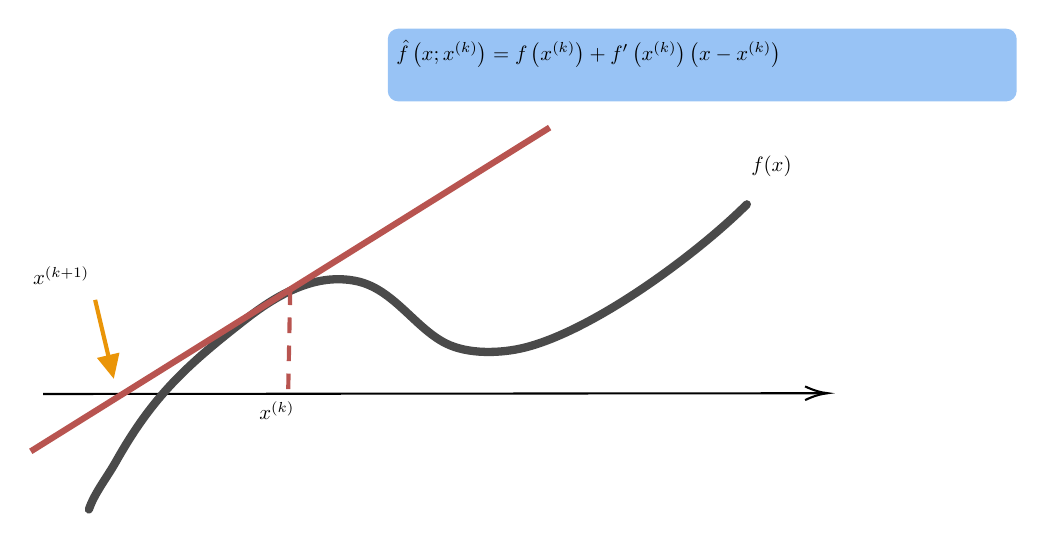
\begin{tikzpicture}[x=0.75pt,y=0.75pt,yscale=-1,xscale=1]
%uncomment if require: \path (0,300); %set diagram left start at 0, and has height of 300

%Straight Lines [id:da987456347938684] 
\draw    (77,220) -- (453,219.62) ;
\draw [shift={(455,219.62)}, rotate = 179.94] [color={rgb, 255:red, 0; green, 0; blue, 0 }  ][line width=0.75]    (10.93,-3.29) .. controls (6.95,-1.4) and (3.31,-0.3) .. (0,0) .. controls (3.31,0.3) and (6.95,1.4) .. (10.93,3.29)   ;
%Shape: Free Drawing [id:dp3634235085264048] 
\draw  [color={rgb, 255:red, 74; green, 74; blue, 74 }  ,draw opacity=1 ][line width=3] [line join = round][line cap = round] (99,275.62) .. controls (101.57,267.9) and (107.73,260.2) .. (112,252.62) .. controls (129.65,221.23) and (145.74,206.38) .. (175,183.62) .. controls (189.89,172.03) and (208.34,161.45) .. (228,165.62) .. controls (245.71,169.37) and (256.02,188.13) .. (271,195.62) .. controls (281.7,200.97) and (297.45,200.51) .. (309,197.62) .. controls (342.7,189.19) and (392.52,152.1) .. (416,128.62) ;
%Straight Lines [id:da8212140101743735] 
\draw [color={rgb, 255:red, 184; green, 84; blue, 80 }  ,draw opacity=1 ][line width=1.5]  [dash pattern={on 5.63pt off 4.5pt}]  (196,169.62) -- (195,219.62) ;
%Straight Lines [id:da6887048674569021] 
\draw [color={rgb, 255:red, 184; green, 84; blue, 80 }  ,draw opacity=1 ][line width=2.25]    (196,169.62) -- (321,91.62) ;
%Straight Lines [id:da06334358045468957] 
\draw [color={rgb, 255:red, 184; green, 84; blue, 80 }  ,draw opacity=1 ][line width=2.25]    (71,247.62) -- (196,169.62) ;
%Straight Lines [id:da7554536985475104] 
\draw [color={rgb, 255:red, 234; green, 149; blue, 8 }  ,draw opacity=1 ][fill={rgb, 255:red, 184; green, 84; blue, 80 }  ,fill opacity=1 ][line width=1.5]    (102,174.65) -- (110.06,208.73) ;
\draw [shift={(110.98,212.62)}, rotate = 256.69] [fill={rgb, 255:red, 234; green, 149; blue, 8 }  ,fill opacity=1 ][line width=0.08]  [draw opacity=0] (11.61,-5.58) -- (0,0) -- (11.61,5.58) -- cycle    ;

% Text Node
\draw (180,222.4) node [anchor=north west][inner sep=0.75pt]  [xscale=0.75,yscale=0.75]  {$x^{( k)}$};
% Text Node
\draw (71,157.4) node [anchor=north west][inner sep=0.75pt]  [xscale=0.75,yscale=0.75]  {$x^{( k+1)}$};
% Text Node
\draw (417,104.4) node [anchor=north west][inner sep=0.75pt]  [xscale=0.75,yscale=0.75]  {$f( x)$};
% Text Node
\draw  [color={rgb, 255:red, 0; green, 0; blue, 0 }  ,draw opacity=0 ][fill={rgb, 255:red, 152; green, 195; blue, 245 }  ,fill opacity=1 ]  (243,49) .. controls (243,46.24) and (245.24,44) .. (248,44) -- (541,44) .. controls (543.76,44) and (546,46.24) .. (546,49) -- (546,74) .. controls (546,76.76) and (543.76,79) .. (541,79) -- (248,79) .. controls (245.24,79) and (243,76.76) .. (243,74) -- cycle  ;
\draw (246,48.4) node [anchor=north west][inner sep=0.75pt]  [xscale=0.75,yscale=0.75]  {$\hat{f}\left( x;x^{(k)}\right) =f\left( x^{(k)}\right) +f^{\prime }\left( x^{(k)}\right)\left( x-x^{(k)}\right)$};


\end{tikzpicture}
\end{FigureCenter}

\subsection{高斯-牛顿法的问题}

然而, $ \hat{f}\left(x ; x^{(k)}\right) $ 只是 $ f(x) $ 的局部近似,仍然可能会有

\begin{remark}
    存在
$$
\left\|f\left(x^{(k+1)}\right)\right\|_{2}^{2}>\left\|f\left(x^{(k)}\right)\right\|_{2}^{2}
$$

的情况。
\end{remark}


Jacobian矩阵Df $ \left(x^{(k)}\right) $ 的可能 "列向量是线性相关。

\begin{remark}
    此时$ \left(D f\left(x^{(k)}\right)^{T} D f\left(x^{(k)}\right)\right) $ 奇异,不可逆。
\end{remark}



\section{Levenberg–Marquardt Algorithm}

Levenberg-Marquardt(LM)算法解决高斯-牛顿法的两个难点:

\begin{enumerate}
    \item 当列 $ D f\left(x^{(k)}\right) $ 是线性相关时,如何更新 $ x^{(k)} $ ?
    \item 当高斯-牛顿法的更新过程, $ \|f(x)\|_{2}^{2} $ 并没有减少。
\end{enumerate}

\subsection{推导Levenberg–Marquardt算法}

LM算法通过求解正则化最小二乘法更新 $ x^{(k+1)} $ :

\begin{problem}
    $$
    x^{(k+1)}=\arg \min _{x}\left\|\hat{f}\left(x ; x^{(k)}\right)\right\|_{2}^{2}+\lambda^{(k)}\left\|x-x^{(k)}\right\|_{2}^{2}
    $$

要求 $ x $ 靠近 $ x^{(k)} $ ,即 $ \hat{f}\left(x ; x^{(k)}\right) \approx f(x) $. (The second term forces $ x $ to be close to $ x^{(k)} $ where $ \hat{f}\left(x ; x^{(k)}\right) \approx f(x) $.)
\end{problem}

当 $ \lambda^{(k)}>0 $ 时,总有唯一解.

\begin{remark}
    Levenberg–Marquardt Algorithm无需再对 $Df \left(x^{(k)}\right) $ 限制。
\end{remark}

\begin{problem}
    第 $ k $ 次迭代求解的最小二乘正则化问题:
$$
x^{(k+1)}=\arg \min _{x}\left\|f\left(x^{(k)}\right)+D f\left(x^{(k)}\right)\left(x-x^{(k)}\right)\right\|_{2}^{2}+\lambda^{(k)}\left\|x-x^{(k)}\right\|_{2}^{2}
$$
\end{problem}



令目标函数导数等于 0 :
$$
\begin{aligned}
    & 2Df\left( x^{(k)}\right)^{T}\left( f\left( x^{(k)}\right) +Df\left( x^{(k)}\right)\left( x-x^{(k)}\right)\right) +2\lambda ^{(k)}\left( x-x^{(k)}\right) =0\\
   \Rightarrow  & \left( Df\left( x^{(k)}\right)^{T} Df\left( x^{(k)}\right) +\lambda ^{(k)} I\right)\left( x-x^{(k)}\right) =-Df\left( x^{(k)}\right)^{T} f\left( x^{(k)}\right)
   \end{aligned}
$$

$ x^{(k+1)} $ 更新:
$$
x^{(k+1)}=x^{(k)}-\left(D f\left(x^{(k)}\right)^{T} D f\left(x^{(k)}\right)+\lambda^{(k)} I\right)^{-1} D f\left(x^{(k)}\right)^{T} f\left(x^{(k)}\right)
$$

\begin{theorem}
    LM算法步骤 $ \Delta x^{(k)}=x^{(k+1)}-x^{(k)} $ 是:

$$ \begin{aligned} \Delta x^{(k)} &=-\left(D f\left(x^{(k)}\right)^{T} D f\left(x^{(k)}\right)+\lambda^{(k)} I\right)^{-1} D f\left(x^{(k)}\right)^{T} f\left(x^{(k)}\right) \\ &=-\frac{1}{2}\left(D f\left(x^{(k)}\right)^{T} D f\left(x^{(k)}\right)+\lambda^{(k)} I\right)^{-1} \nabla g\left(x^{(k)}\right) \end{aligned} $$
\end{theorem}

\begin{theorem}
    对于 $ \lambda^{(k)}=0 $ ,简化为高斯-牛顿法
\end{theorem}

\begin{theorem}
    对于较大的 $ \lambda^{(k)} $ :
$$
\Delta x^{(k)} \approx-\frac{1}{2 \lambda^{(k)}} \nabla g\left(x^{(k)}\right)
$$
\end{theorem}



\subsection{正则化参数}

几种调整 $ \lambda^{(k)} $ 的策略.

\begin{algorithm}[htbp]
    \caption{在第$k$次迭代时,求解$\hat{x}$}
    $$
    \hat{x}=\arg \min _{x}\left\|\hat{f}\left(x ; x^{(k)}\right)\right\|_{2}^{2}+\lambda^{(k)}\left\|x-x^{(k)}\right\|_{2}^{2}
    $$\;
    

    \If(){$ \|f(\hat{x})\|_{2}^{2}<\left\|f\left(x^{(k)}\right)\right\|_{2}^{2} $}{
        $ x^{(k+1)}=\hat{x} $\;
        降低 $ \lambda $
    }
    \Else(){
        无需更新 $ x \left(x^{(k+1)}=x^{(k)}\right) $\;
        增加 $ \lambda $\;

    }
\end{algorithm}

它的一些变化:

\begin{example}
    比较预期损失降低的情况和实际损失降低的情况。(compare actual cost reduction with predicted cost reduction)
\end{example}

\begin{theorem}
    在第$k$次迭代时,求解$\hat{x}$

    $$
    \hat{x}=\arg \min _{x}\left\|\hat{f}\left(x ; x^{(k)}\right)\right\|_{2}^{2}+\lambda^{(k)}\left\|x-x^{(k)}\right\|_{2}^{2}
    $$

    等价于

    具有“置信区间”的最小二乘法问题:
    $ \min _{x}\left\|\hat{f}\left(x ; x^{(k)}\right)\right\|_{2}^{2} $
    subject to $ \left\|x-x^{(k)}\right\|_{2}^{2} \leq \gamma $
\end{theorem}


\begin{algorithm}[htbp]
    \caption{Levenberg–Marquardt Algorithm}
    选择 $ x^{(1)} $ 和 $ \lambda^{(1)} $\;
    \While{$ k=1,2, \ldots $}{
        求 $ f\left(x^{(k)}\right) $\;
        $ A=D f\left(x^{(k)}\right) $\;
        计算最小二乘法正则化问题的解:
        $$
        \hat{x}=x^{(k)}-\left(A^{T} A+\lambda^{(k)} I\right)^{-1} A^{T} f\left(x^{(k)}\right)
        $$\;
        计算 $ x^{(k+1)} $ 和 $ \lambda^{(k+1)} $ :
        $$\displaystyle \left\{\begin{array}{ c c c }
        x^{(k+1)} =\hat{x} , & \lambda ^{(k+1)} =\beta _{1} \lambda ^{(k)} & \left(\text{if} \ \| (\hat{x} )\| _{2}^{2} < \left\Vert f\left( x^{(k)}\right)\right\Vert _{2}^{2}\right)\\
        x^{(k+1)} =x^{(k)} , & \lambda ^{(k+1)} =\beta _{2} \lambda ^{(k)} & \left(\text{others}\right)
        \end{array}\right. $$\;

    }
\end{algorithm}

\begin{itemize}
    \item 其中 $ \beta_{1}, \beta_{2} $ 是常数, $ 0<\beta_{1}<1<\beta_{2} $ 。
    \item 在步骤2中,可以使用 $ \mathrm{QR} $ 分解来计算 $ \hat{x} $ 。
    \item 迭代会在当 $ \nabla g\left(x^{(k)}\right)=2 A^{T} f\left(x^{(k)}\right) $ 足够小时终止。
\end{itemize}

\section{Newton Method}

\begin{proposition}
    Assume $ f: \mathbf{R}^{n} \rightarrow \mathbf{R}^{n} $ is differentiable.
\end{proposition}



\begin{algorithm}
    \caption{Newton's Method}
     choose $ x^{(1)} $\;
     \While{$ k=1,2, \ldots $}{
         $$
        x^{(k+1)}=x^{(k)}-D f\left(x^{(k)}\right)^{-1} f\left(x^{(k)}\right)
        $$\;
     }
\end{algorithm}



$ D f\left(x^{(k)}\right) $ is the derivative matrix of $ f $ at $ x^{(k)} $. 

Each iteration requires one evaluation of $ f(x) $ and $ D f(x) $, each iteration requires factorization of the $ n \times n $ matrix $ D f(x) $.

\begin{proposition}
    We assume $ D f(x) $ is nonsingular.
\end{proposition}

\subsection{Interpretation of Newton Method}

$$
x^{(k+1)}=x^{(k)}-D f\left(x^{(k)}\right)^{-1} f\left(x^{(k)}\right)
$$

linearize $ f $ (i.e., make affine approximation) around current iterate $ x^{(k)} $
$$
\hat{f}\left(x ; x^{(k)}\right)=f\left(x^{(k)}\right)+D f\left(x^{(k)}\right)\left(x-x^{(k)}\right)
$$

solve the linearized equation $ \hat{f}\left(x ; x^{(k)}\right)=0 $; the solution is
$$
x=x^{(k)}-D f\left(x^{(k)}\right)^{-1} f\left(x^{(k)}\right)
$$

take the solution $ x $ of the linearized equation as the next iterate $ x^{(k+1)} $

\subsection{One Variable}

\begin{FigureCenter}{$m=n=1$时的情形}

    \tikzset{every picture/.style={line width=0.75pt}} %set default line width to 0.75pt        
    
    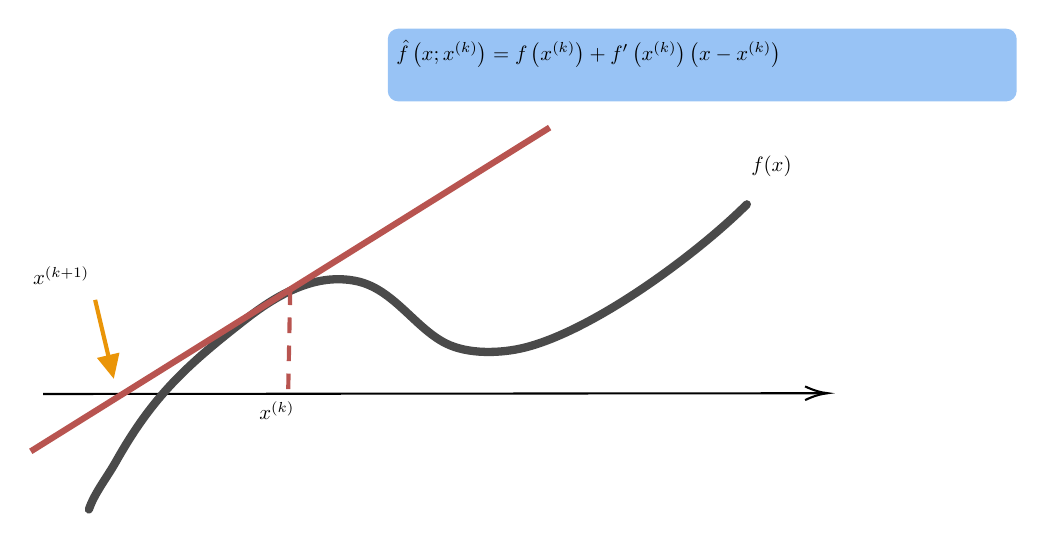
\begin{tikzpicture}[x=0.75pt,y=0.75pt,yscale=-1,xscale=1]
    %uncomment if require: \path (0,300); %set diagram left start at 0, and has height of 300
    
    %Straight Lines [id:da987456347938684] 
    \draw    (77,220) -- (453,219.62) ;
    \draw [shift={(455,219.62)}, rotate = 179.94] [color={rgb, 255:red, 0; green, 0; blue, 0 }  ][line width=0.75]    (10.93,-3.29) .. controls (6.95,-1.4) and (3.31,-0.3) .. (0,0) .. controls (3.31,0.3) and (6.95,1.4) .. (10.93,3.29)   ;
    %Shape: Free Drawing [id:dp3634235085264048] 
    \draw  [color={rgb, 255:red, 74; green, 74; blue, 74 }  ,draw opacity=1 ][line width=3] [line join = round][line cap = round] (99,275.62) .. controls (101.57,267.9) and (107.73,260.2) .. (112,252.62) .. controls (129.65,221.23) and (145.74,206.38) .. (175,183.62) .. controls (189.89,172.03) and (208.34,161.45) .. (228,165.62) .. controls (245.71,169.37) and (256.02,188.13) .. (271,195.62) .. controls (281.7,200.97) and (297.45,200.51) .. (309,197.62) .. controls (342.7,189.19) and (392.52,152.1) .. (416,128.62) ;
    %Straight Lines [id:da8212140101743735] 
    \draw [color={rgb, 255:red, 184; green, 84; blue, 80 }  ,draw opacity=1 ][line width=1.5]  [dash pattern={on 5.63pt off 4.5pt}]  (196,169.62) -- (195,219.62) ;
    %Straight Lines [id:da6887048674569021] 
    \draw [color={rgb, 255:red, 184; green, 84; blue, 80 }  ,draw opacity=1 ][line width=2.25]    (196,169.62) -- (321,91.62) ;
    %Straight Lines [id:da06334358045468957] 
    \draw [color={rgb, 255:red, 184; green, 84; blue, 80 }  ,draw opacity=1 ][line width=2.25]    (71,247.62) -- (196,169.62) ;
    %Straight Lines [id:da7554536985475104] 
    \draw [color={rgb, 255:red, 234; green, 149; blue, 8 }  ,draw opacity=1 ][fill={rgb, 255:red, 184; green, 84; blue, 80 }  ,fill opacity=1 ][line width=1.5]    (102,174.65) -- (110.06,208.73) ;
    \draw [shift={(110.98,212.62)}, rotate = 256.69] [fill={rgb, 255:red, 234; green, 149; blue, 8 }  ,fill opacity=1 ][line width=0.08]  [draw opacity=0] (11.61,-5.58) -- (0,0) -- (11.61,5.58) -- cycle    ;
    
    % Text Node
    \draw (180,222.4) node [anchor=north west][inner sep=0.75pt]  [xscale=0.75,yscale=0.75]  {$x^{( k)}$};
    % Text Node
    \draw (71,157.4) node [anchor=north west][inner sep=0.75pt]  [xscale=0.75,yscale=0.75]  {$x^{( k+1)}$};
    % Text Node
    \draw (417,104.4) node [anchor=north west][inner sep=0.75pt]  [xscale=0.75,yscale=0.75]  {$f( x)$};
    % Text Node
    \draw  [color={rgb, 255:red, 0; green, 0; blue, 0 }  ,draw opacity=0 ][fill={rgb, 255:red, 152; green, 195; blue, 245 }  ,fill opacity=1 ]  (243,49) .. controls (243,46.24) and (245.24,44) .. (248,44) -- (541,44) .. controls (543.76,44) and (546,46.24) .. (546,49) -- (546,74) .. controls (546,76.76) and (543.76,79) .. (541,79) -- (248,79) .. controls (245.24,79) and (243,76.76) .. (243,74) -- cycle  ;
    \draw (246,48.4) node [anchor=north west][inner sep=0.75pt]  [xscale=0.75,yscale=0.75]  {$\hat{f}\left( x;x^{(k)}\right) =f\left( x^{(k)}\right) +f^{\prime }\left( x^{(k)}\right)\left( x-x^{(k)}\right)$};
    
    
    \end{tikzpicture}
    \end{FigureCenter}

affine approximation of $ f $ around $ x^{(k)} $ is
$$
\hat{f}\left(x ; x^{(k)}\right)=f\left(x^{(k)}\right)+f^{\prime}\left(x^{(k)}\right)\left(x-x^{(k)}\right)
$$

solve the linearized equation $ \hat{f}\left(x ; x^{(k)}\right)=0 $ and take the solution as $ x^{(k+1)} $ :
$$
x^{(k+1)}=x^{(k)}-\frac{f\left(x^{(k)}\right)}{f^{\prime}\left(x^{(k)}\right)}
$$

\subsection{Relation to Gauss–Newton method}

recall Gauss-Newton method for nonlinear least squares problem

\begin{problem}[nonlinear least squares problem]
    $$\term{minimize} \quad\|f(x)\|^{2} $$
\end{problem}

where $ f $ is a differentiable function from $ \mathbf{R}^{n} $ to $ \mathbf{R}^{m} $.

Gauss-Newton update
$$
x^{(k+1)}=x^{(k)}-\left(D f\left(x^{(k)}\right)^{T} D f\left(x^{(k)}\right)\right)^{-1} D f\left(x^{(k)}\right)^{T} f\left(x^{(k)}\right)
$$

If $ m=n $, then $ D f(x) $ is square and this is the Newton update
$$
x^{(k+1)}=x^{(k)}-D f\left(x^{(k)}\right)^{-1} f\left(x^{(k)}\right)
$$

\subsection{Examples}

\begin{example}
    % todo (2021-12-10 07:54): figure
    $$ f_{1}\left(x_{1}, x_{2}\right)=\log \left(x_{1}^{2}+2 x_{2}^{2}+1\right)-0.5=0 $$
$$ f_{2}\left(x_{1}, x_{2}\right)=x_{2}-x_{1}^{2}+0.2=0 $$

two equations in two variables; two solutions $ (0.70,0.29),(-0.70,0.29) $.

Newton iteration

\begin{algorithm}[htbp]
    \caption{Newton iteration}
    evaluate $ g=f(x) $ and
$$
H=D f(x)=\left[\begin{array}{cc}
2 x_{1} /\left(x_{1}^{2}+2 x_{2}^{2}+1\right) & 4 x_{2} /\left(x_{1}^{2}+2 x_{2}^{2}+1\right) \\
-2 x_{1} & 1
\end{array}\right]
$$\;
solve $ H v=-g $ (two linear equations in two variables)\;
update $ x:=x+v $\;
\end{algorithm}


Results: 

\begin{itemize}
    \item $ x^{(1)}=(1,1) $ : converges to $ x^{\star}=(0.70,0.29) $ in about 4 iterations
    \item $ x^{(1)}=(-1,1) $ : converges to $ x^{\star}=(-0.70,0.29) $ in about 4 iterations
    \item $ x^{(1)}=(1,-1) $ or $ x^{(0)}=(-1,-1): $ does not converge
\end{itemize}

\end{example}

\begin{itemize}
    \item Newton's method works very well if started near a solution, may not work otherwise
    \item can converge to different solutions depending on the starting point
    \item does not necessarily find the solution closest to the starting point
\end{itemize}

\subsection{Convergence of Newton's method}

Quadratic convergence explains fast convergence when started near solution.

\begin{theorem}[Quadratic Convergence]
    if $ f\left(x^{\star}\right)=0 $ and $ D f\left(x^{\star}\right) $ is nonsingular, and $ x^{(1)} $ is sufficiently close to $ x^{\star} $, then
$$
x^{(k)} \rightarrow x^{\star}, \quad\left\|x^{(k+1)}-x^{\star}\right\| \leq c\left\|x^{(k)}-x^{\star}\right\|^{2}
$$
for some $ c>0 $
\end{theorem}

\subsection{Newton's method for minimizing a convex function}

if $ \nabla^{2} g(x) $ is positive definite everywhere, we can minimize $ g(x) $ by solving
$$
\nabla g(x)=0
$$


Algorithm:
\begin{algorithm}[htbp]
    \caption{Newton's method for minimizing a convex function}
    choose $ x^{(1)} $\;
    \While(){$ k=1,2, \ldots $}{
        $$
x^{(k+1)}=x^{(k)}-\nabla^{2} g\left(x^{(k)}\right)^{-1} \nabla g\left(x^{(k)}\right)
$$\;
    }
\end{algorithm}

$ v=-\nabla^{2} g(x)^{-1} \nabla g(x) $ is called the Newton step at $ x $.

It converges if started sufficiently close to the solution. Newton step is computed by a Cholesky factorization of the Hessian.

\subsubsection{Interpretations of Newton step}


\begin{definition}[affine approximation of $ f(x)=\nabla g(x) $ around $ x^{(k)} $]
    $$
\hat{f}\left(x ; x^{(k)}\right)=\nabla g\left(x^{(k)}\right)+\nabla^{2} g\left(x^{(k)}\right)\left(x-x^{(k)}\right)
$$
\end{definition} is

Newton update $ x^{(k+1)} $ is solution of linear equation $ \hat{f}\left(x ; x^{(k)}\right)=0 $.

\begin{definition}[quadratic approximation of $ g(x) $ around $ x^{(k)} $]
    $$
g_{\mathrm{q}}\left(x ; x^{(k)}\right)=g\left(x^{(k)}\right)+\nabla g\left(x^{(k)}\right)^{T}\left(x-x^{(k)}\right)+\frac{1}{2}\left(x-x^{(k)}\right)^{T} \nabla^{2} g\left(x^{(k)}\right)\left(x-x^{(k)}\right)
$$
\end{definition}

Newton update $ x^{(k+1)} $ minimizes $ g_{\mathrm{q}}\left(x ; x^{(k)}\right)\left(\right. $ satisfies $ \left.\nabla g_{\mathrm{q}}\left(x ; x^{(k)}\right)=0\right) $

% todo (2021-12-10 08:48): figure

\subsection{Damped Newton method}

\begin{algorithm}
    \caption{Damped Newton method}
    choose $ x^{(1)} $\;
    \While(){$ k=1,2, \ldots $}{
        compute Newton step $ v=-\nabla^{2} g\left(x^{(k)}\right)^{-1} \nabla g\left(x^{(k)}\right) $\;
        (Line Search) find largest $ t $ in $ \left\{1,0.5,0.5^{2}, 0.5^{3}, \ldots\right\} $ that satisfies
        $$
        g\left(x^{(k)}+t v\right)<g\left(x^{(k)}\right)
        $$\;
        $ x^{(k+1)}=x^{(k)}+t v $\;
    }
\end{algorithm}

Positive scalar $ t $ is called the \term{step size}, step 2 in algorithm is called \term{line search}.

\subsubsection{Interpretation of line search} 

to determine a suitable step size, consider the function $ h: \mathbf{R} \rightarrow \mathbf{R} $
$$
h(t)=g\left(x^{(k)}+t v\right)
$$

% todo (2021-12-10 08:49): figure

$ h^{\prime}(0)=\nabla g\left(x^{(k)}\right)^{T} v $ is the directional derivative at $ x^{(k)} $ in the direction $ v $

line search terminates with positive $ t $ if $ h^{\prime}(0)<0 $ ( $ v $ is a descent direction)

if $ \nabla^{2} g\left(x^{(k)}\right) $ is positive definite, the Newton step is a descent direction
$$
h^{\prime}(0)=\nabla g\left(x^{(k)}\right)^{T} v=-v^{T} \nabla^{2} g\left(x^{(k)}\right) v<0
$$

\subsubsection{Newton method for nonconvex functions}

if $ \nabla^{2} g\left(x^{(k)}\right) $ is not positive definite, it is possible that Newton step $ v $ satisfies
$$
\nabla g\left(x^{(k)}\right)^{T} v=-\nabla g\left(x^{(k)}\right)^{T} \nabla^{2} g\left(x^{(k)}\right)^{-1} \nabla g\left(x^{(k)}\right)>0
$$

% todo (2021-12-10 08:50): figure

- if Newton step is not descent direction, replace it with descent direction
- simplest choice is $ v=-\nabla g\left(x^{(k)}\right) $; practical methods make other choices

\section{Newton method for nonlinear least squares}

\subsection{Hessian of nonlinear least squares cost}

$$
g(x)=\|f(x)\|^{2}=\sum_{i=1}^{m} f_{i}(x)^{2}
$$

\begin{theorem}
   gradient:

$$
\nabla g(x)=2 \sum_{i=1}^{m} f_{i}(x) \nabla f_{i}(x)=2 D f(x)^{T} f(x)
$$ 
\end{theorem}

\begin{theorem}
    second derivatives:
$$
\frac{\partial^{2} g}{\partial x_{j} \partial x_{k}}(x)=2 \sum_{i=1}^{m}\left(\frac{\partial f_{i}}{\partial x_{j}}(x) \frac{\partial f_{i}}{\partial x_{k}}(x)+f_{i}(x) \frac{\partial^{2} f_{i}}{\partial x_{j} \partial x_{k}}(x)\right)
$$
\end{theorem}

\begin{theorem}
    Hessian
$$
\nabla^{2} g(x)=2 D f(x)^{T} D f(x)+2 \sum_{i=1}^{m} f_{i}(x) \nabla^{2} f_{i}(x)
$$
\end{theorem}

\begin{theorem}
    (Undamped) Newton step at $ x=x^{(k)} $ :
$$
\begin{aligned}
v_{\mathrm{nt}} &=-\nabla^{2} g(x)^{-1} \nabla g(x) \\
&=-\left(D f(x)^{T} D f(x)+\sum_{i=1}^{m} f_{i}(x) \nabla^{2} f_{i}(x)\right)^{-1} D f(x)^{T} f(x)
\end{aligned}
$$

\end{theorem}

\begin{theorem}
    Gauss-Newton step at $ x=x^{(k)} $
$$
v_{\mathrm{gn}}=-\left(D f(x)^{T} D f(x)\right)^{-1} D f(x)^{T} f(x)
$$
\end{theorem}

\begin{corollary}
    can be written as $ v_{\mathrm{gn}}=-H_{\mathrm{gn}}^{-1} \nabla g(x) $ where $ H_{\mathrm{gn}}=2 D f(x)^{T} D f(x) $

    $ H_{\mathrm{gn}} $ is the Hessian without the term $ \sum_{i} f_{i}(x) \nabla^{2} f_{i}(x) $.
\end{corollary}





\subsection{Comparison}

Newton step:
\begin{itemize}
    \item requires second derivatives of $ f $
    \item not always a descent direction $ \left(\nabla^{2} g(x)\right. $ is not necessarily positive definite)
    \item fast convergence near local minimum
\end{itemize}


Gauss-Newton step:
\begin{itemize}
    \item does not require second derivatives
    \item a descent direction (if columns of $ D f(x) $ are linearly independent):
    $$
    \nabla g(x)^{T} v_{\mathrm{gn}}=-2 v_{\mathrm{gn}}^{T} D f(x)^{T} D f(x) v_{\mathrm{gn}}<0 \quad \text { if } v_{\mathrm{gn}} \neq 0
    $$
    \item local convergence to $ x^{\star} $ is similar to Newton method if
$$
\sum_{i=1}^{m} f_{i}\left(x^{\star}\right) \nabla^{2} f_{i}\left(x^{\star}\right)
$$
is small (e.g., $ f\left(x^{\star}\right) $ is small, or $ f $ is nearly affine around $ x^{\star} $ )
\end{itemize}


\section{Unconstrained minimization problem}

\begin{problem}
    Assume that $ g $ is twice differentiable

    $\text{minimize} \quad g\left(x_{1}, x_{2}, \ldots, x_{n}\right) $

    $ g $ is a function from $ \mathbf{R}^{n} $ to $ \mathbf{R} $ (the cost function or objective function), $ x=\left(x_{1}, x_{2}, \ldots, x_{n}\right) $ is $ n $-vector of optimization variables.
\end{problem}

to solve a maximization problem (i.e., maximize $ g(x) $ ), minimize $ -g(x) $.

\section{Local and global optimum}

\begin{definition}[globally optimal]
    $ x^{\star} $ is an optimal point (or a minimum) if
$$
g\left(x^{\star}\right) \leq g(x) \quad \text { for all } x
$$

It is also called globally optimal.
\end{definition}

\begin{definition}[locally optimal]
    $ x^{\star} $ is a locally optimal point (local minimum) if for some $ R>0 $
$ g\left(x^{\star}\right) \leq g(x) \quad $ for all $ x $ with $ \left\|x-x^{\star}\right\| \leq R $

    It is also called locally optimal.
\end{definition}





